\chapter{Gateway}
A gateway is a device that forwards messages from another device, the client, to a second device, the server or another gateway.
In the following figures, there are two examples of gateways: Layer-3 gateways (routers in Section \ref{router_section}) and Layer-7 gateways (proxy).
\begin{figure}[h]
\centering
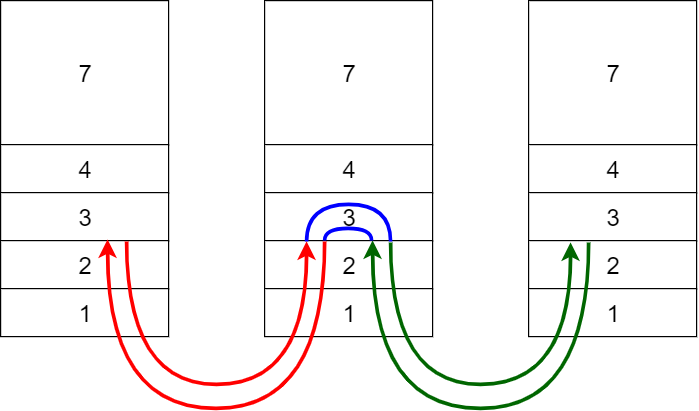
\includegraphics[scale=0.4]{Images/Gateway/gateway_3}
\caption{\footnotesize{Router (Layer-3 gateway).}}\label{gateway_3}
\end{figure}
\begin{figure}[h]
\centering
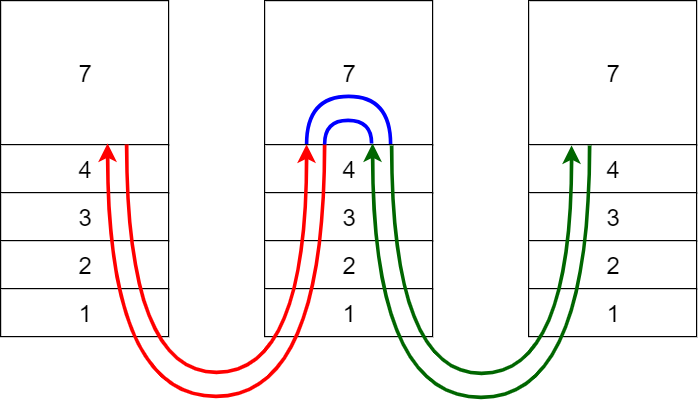
\includegraphics[scale=0.4]{Images/Gateway/gateway_7}
\caption{\footnotesize{Proxy (Layer-7 gateway).}}\label{gateway_7}
\end{figure}

\section{Proxy}
A Layer-7 gateway is also called proxy. It works as an intermediary between two identical protocols (Figure \ref{proxy}). Instead of Layer-3 gateways, proxy can also see the full stream of data, analyze HTTP headers and implement new functions. 
\begin{figure}[h]
\centering
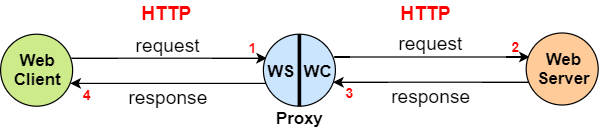
\includegraphics[scale=0.42]{Images/Gateway/proxy}
\caption{\footnotesize{Example of proxy use.}}\label{proxy}
\end{figure}
The main possible functions are:
\begin{itemize}
\item{\textbf{Caching}\\
It's used to reduce traffic directed to the server. The proxy does the most expensive job, managing all the requests of the same page of the server. \\
After the request of the page for the first time, the proxy asks the page to the server and then stores in its system, before replying. Hence the next clients requests of the same page will be manage only by proxy because the page was already stored in its system.\\
In this case the server needs to manage only a request by proxy and provide a response to proxy.
\begin{figure}[h]
\centering
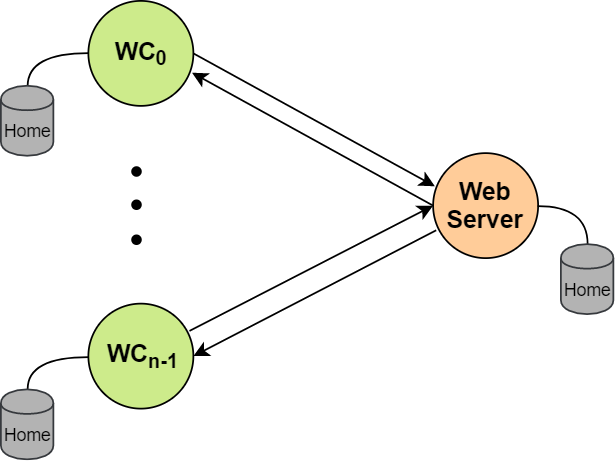
\includegraphics[scale=0.38]{Images/Gateway/proxy_cache_no}
\caption{\footnotesize{Example of caching without proxy.}}\label{proxy_cache_no}
\end{figure}
\begin{figure}[h]
\centering
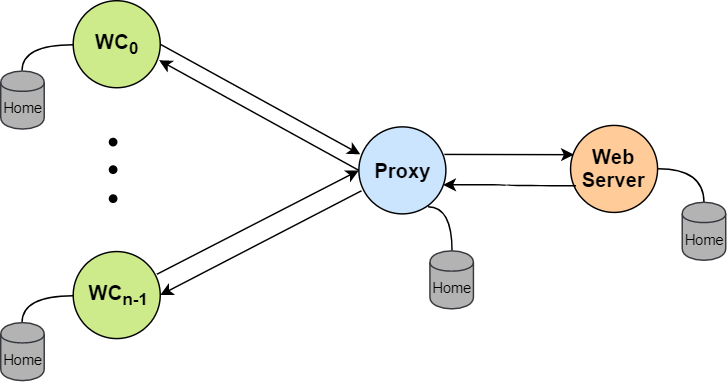
\includegraphics[scale=0.4]{Images/Gateway/proxy_cache}
\caption{\footnotesize{Example of caching using proxy.}}\label{proxy_cache}
\end{figure}
}
\item{\textbf{Filtering}\\
The proxy can do two actions:
\begin{itemize}
\item{\textbf{Filtering the requested resource by the client}\\
there are many companies that doesn't give access to some services (E.g. no access to Facebook, Youtube, ...).\\
We cannot use a filtering approach at lower levels because in some cases clients can access to services through intermediate addresses, different from the one we want to reach. Hence we need to analyze the HTTP request at upper layer.}
\item{\textbf{Filtering the content of the response}\\
for parent control approach.}
\end{itemize}
\begin{figure}[h]
\centering
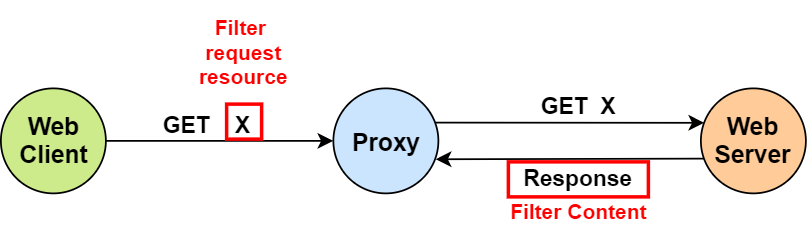
\includegraphics[scale=0.4]{Images/Gateway/proxy_filter}
\caption{\footnotesize{Example of proxy filtering.}}\label{proxy_filter}
\end{figure}
}
\item{\textbf{Web Application Firewall (WAF)}\\
The proxy is specialized and used to block suspicious requests. This is done by analyzing request content, looking for not secure pattern.\\
A possible pattern can be \textit{".."} in the path of the resource, that could give access to not accessible part of the File System (injection). Another possible pattern could be a suspicious parameter for a web application to manage SQL database (SQL injection).
\begin{figure}[h]
\centering
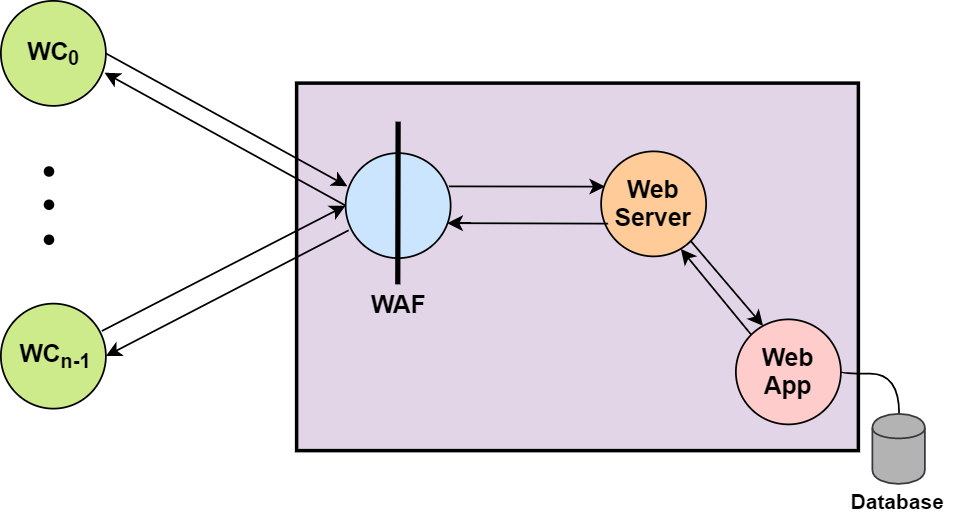
\includegraphics[scale=0.4]{Images/Gateway/proxy_waf}
\caption{\footnotesize{Example of WAF use.}}\label{proxy_waf}
\end{figure}
}
\item{\textbf{Load Balancing}\\
The proxy is a load balancer for the clients requests to the server.\\
There are many servers to manage requests by client. The client makes the request of the web page but in the reality it's talking with the proxy, that manage the request by sending it to a particular server.\\
This action is repeated for each client's request. Hence the client thinks that is talking to one server but in reality, the proxy distribute the requests among several servers. 
\begin{figure}[h]
\centering
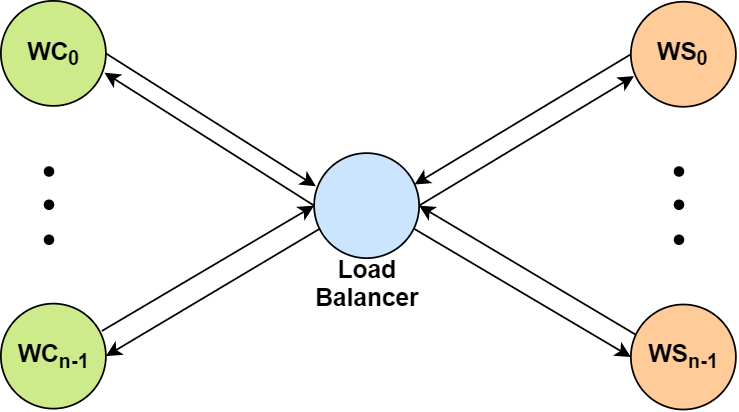
\includegraphics[scale=0.4]{Images/Gateway/proxy_load}
\caption{\footnotesize{Example of load balancing through proxy.}}\label{proxy_load}
\end{figure}
}
\end{itemize}

\section{Router} \label{router_section}
A router is a device that does two main functions:
\begin{enumerate}
\item{\textbf{Routing}\\
it decides on which outbound link send the packet. This decision is based on destination address and its router table (Table \ref{routing_table}). In each routing table, a network address is associated to an outbound interface, where the packet will be forwarded.\\
Each network address is followed by a \textbf{"/"} and a number that defines how many most significant bits of \textbf{net mask} are set to 1. The default adddress, that is always in each routing table, is \textbf{0.0.0.0}. This one is associated to the interface on which the packet will be sent if no one of the previous messages matches with the one of the destination.\\
For each entry of the routing table, the network address is ANDed with its net mask and the IP address, we are looking for, ANDed with that net mask gives us the same result of the first one, the packet is sent to the corresponding interface.\\
The default address \textbf{0.0.0.0} is associated with a net mask, composed by all 0's. Hence every address, ANDed with this net mask, matches with default address \textbf{0.0.0.0}.
\begin{table}[h]
\centering \footnotesize
\begin{tabular}{|c|c|}
\hline
\textbf{Address prefix} & \textbf{Outbound interface}\\
\hline
{147.162.0.0\textit{/16}} & {2}\\
{88.80.187.0\textit{/24}} & {4}\\
{...} & {...}\\
{0.0.0.0} & {1}\\
\hline
\end{tabular}
\caption{Example of a routing table.}\label{routing_table}
\end{table}
}
\item{\textbf{Switching}\\
it sends the packet to the link previously selected.}
\end{enumerate}
Each router manages all the incoming packets, storing them in a input \textbf{FIFO buffer} (\textit{Standard Service Layer}). By default, if packets arrive too fast to in the buffer, w.r.t. velocity of incoming data processing, new packets are dropped if buffer is already full according to some policy (Figure \ref{SEEEEEEEEE}).\\
Hence routers has not responsability if some packets are dropped because of it declares it in advance and its goal is to give user the best effort. The behaviour of the router management of the input buffer is based on different policy, according to a goal:\\
\begin{itemize}
\item{\textit{To reduce} \textbf{latency}\\
the packets are sorted by precedence index
}
\item{\textit{To reduce} \textbf{loss rate}\\
dropped packets are the last enetered without \textit{R} bit set
}
\item{\textit{To reduce} \textbf{throughput}\\
the packets are stored by index, calculated by the router, based on the amount of data transfered from each source/destination in a time unit (e.g. RSUP, virtual clock, MPLS, Stop \& GO criteria)
}
\end{itemize}
The user cannot set all the possible criteria, because these depend from agreement developed with Service Provider. Hence the Internet Service Provider, if all criteria are set, reset them all before sending packets to Internet.